\chapter{Einleitung}
Die Astrophysik zeichnet aus, dass, im Gegensatz zu Laborexperimenten, diese ihre Observablen nicht gezielt beeinflussen kann.
Somit ist sie angewiesen, die begrenzten kosmischen Experimente ihrer Zeit passiv zu beobachten. 
Dabei übernimmt das FACT Teleskop die Aufgabe, mehrere kosmische Strahlungsquellen zu beobachten und bei Anomalitäten größere Teleskope, für die genauere Observation der Ereignissen, zu informieren. 

Im Feld der Astroteilchenphysik werden verschiedene Quellen im Weltraum observiert.
Ziel der Observation ist, ein tiefgreifendes Verständinis über die Entstehung sowie die dominierenden Wechselwikungsprozesse zu erlangen. 
Quellen kosmischer Strahlung sind überwiegend aktive galaktische Kerne, Neutronensterne und Supernova-Überreste. 
Die Energie der Teilchen decken ein Spektrum von \SI{e7}{\electronvolt} bei solarer kosmischer Strahlung bis zu \SI{e20}{\electronvolt} bei extragalaktischer kosmischer Strahlung ab. 

\begin{figure}
  \centering
  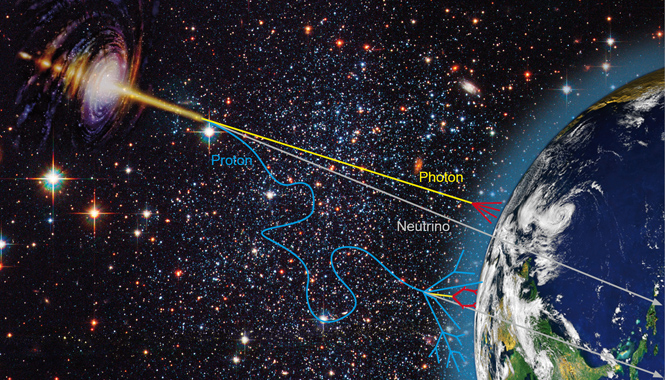
\includegraphics[width=0.6\textwidth]{./images/sources-detection.jpg}
  \caption{Möglicher Weg der dreier Klassen von Teilchen von der Quelle bis zu ihrer Detektion \cite{overview-detec}.}
\end{figure}

Bei ihrem Weg von der Quelle durchs Universum treffen auf die Atmosphäre der Erde durchschnittlich \SI{1e5}{\per\second\per\meter\squared} Teilchen.
Diese produzieren je nach Teilchenart und Energie weitere Schauer, in denen viele weitere Sekundärteilchen erzeugt werden. 
Je nach Teilchenart gibt es verschiedene Detektionsmöglichkeiten, wovon das FACT eine erdbasierte Variante für $\gamma$-Quanten und Hadronen ist. 
Die verschiedenen kosmischen Teilchen lassen sich in drei verschiedene Klassen einteilen. 
Dabei zählt der Sonnenwind zu einer der ständigen Quellen, durch die geladene kosmische Strahlung auf die Erdatmosphäre trifft.

\section{Neutrinos}
Aufgrund ihrer elektrischen Neutralität sowie ihres geringen Wirkungsquerschnitts liefern Neutrinos Informationen über die Quellregionen. 
Dabei werden diese nicht durch galaktische Magnetfelder beschleunigt, noch geht ihre Richtungsinformation verloren. 
Zum Nachweis von astrophysikalischen Neutrinos werden, aufgrund ihrer geringen Wechselwirkungswahrscheinlichkeit große Detektorvolumina, wie zum Beispiel das IceCube Experiment benötigt.
Da ein direkter Nachweis bis jetzt nicht möglich ist, wird beim IceCube Experiment sich der Cherenkov-Effekt im Eis zu Nutzen gemacht, um über indirekte Strahlung Neutrinos nachzuweisen.


\section{Geladene kosmische Strahlung}
Geladene kosmische Strahlung besteht überwiegend aus Protonen, Heliumkernen und freien Elektronen. 
Aufgrund ihrer Ladung verliert sie jegliche Richtungsinformation durch intergalaktische Magnetfelder. 
Dies hat zur Folge, dass die Erde isotrop von geladener Strahlung ausgeleuchtet wird.
Die geladene Strahlung tritt wesentlich häufiger auf, als die anderen beiden Klassen. 

\section{Photonen}
Photonen sind ebenfalls wie Neutrinos ungeladen, sodass eine Richtungsrekonstruktion mit ihnen möglich ist. 
Jedoch kommt es bei der Detektion auf der Erde zur Schauerbildung, sodass die Richtungsrekonstruktion nicht ganz trivial ist. 
Dies kann umgangen werden, indem Satelliten in die Erdumlaufbahn gebracht werden sodass der Cherenkov-Effekt unterdrückt wird, wie es zum Beispiel beim Fermi Gamma-ray Space Telescope der Fall ist.

